\section{Timing Compartments}
    Timing compartments are a new architecture primitive that control timing 
    channel leakage among software entities that share hardware. When combined 
    with explicit channel protection (such as access controls) timing 
    compartments provide total software isolation.
    A timing compartment consists of one or more software entities. Here a 
    software entitiy is some system abstraction (such as processes or threads 
    in a single OS system or virtual machines in a virtualization based system) 
    that execute software and have an owner.
    
    Timing channels between timing compartments must be controlled according to 
    a policy that meets the security requirements of the system. This policy 
    entails of a lattice of security levels such as $\mathtt{low} \leq
    \mathtt{high}$. A timing compartment can only leak information to a 
    preceeding timing compartment in the lattice. This lattice model is quite 
    expressive. The lattice $\mathtt{low} \leq \mathtt{high}$ defines a policy 
    where a high assurance software entity can not leak information to a low 
    assurance one. The lattice $\mathtt{T_1} \nleq \mathtt{T_2}, \mathtt{T_2} 
    \nleq \mathtt{T_1}$ defines a policy where $T_1$ and $T_2$ are mutually 
    distrusting. By convention, security lables share names with their timing 
    compartments. 
 
    To enforce the policy a trusted software component called the timing 
    compartment manager (TCM) confines software entities into TCs. The TCM then 
    informs the hardware of the TCs and policy. At runtime, the TCM tags 
    hardware requests with a tag to indicate the TC of the software entity that 
    made the request. 

    Timing compartments only address timing channels; they do not control 
    information flow through explicit channels. Handling these concerns 
    separately allows for more flexibility in the overall system design.  When 
    designing a secure system, implementors must consider how the cost required 
    to carry out a particular attack compares with other attacks, the potential 
    damage that could be caused by an attack, and the cost and performance 
    impact of implementing the security mechanisms needed to stop it. This 
    enables timing compartments to provide timing channel protection only to 
    software entities that need it.

    \subsection{Applications}
    This section describes how to apply timing compartments to protect the 
    vulnerable systems described in section \ref{sec:cloud_scenario}.
    \subsubsection{Cloud Computing}
    In the cloud computing system described eariler, VM1 and VM2 are both 
    running applications with high security needs. Both distrust eachother and 
    all other VMs in the system. VM3 and VM4 are running programs that require 
    a lot of performance, but have low security needs. All VMs implicitly trust 
    the hypervisor. Figure \ref{fig:cloud_tcs} shows timing compartments can be 
    applied to meet the needs of this system. VM1 and VM2 are confined to their 
    own timing compartments TC1 and TC2, but VM3 and VM4 are grouped in TC3.  
    The hypervisor is extended with a TCM and confined to TC0 since it also 
    requires timing channel protection. 
    
    \begin{figure}
        \begin{center}
            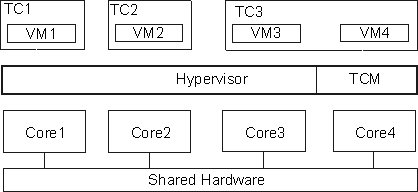
\includegraphics[width=1.51in]{figs/cloud_tcs.pdf}
            \caption{ An application of timing compartments to a cloud 
                computing environment. The hypervisor and high assurance VMs 
                are confined to their own TCs while low assurance VMs share TC3
            }
            \label{fig:cloud_tcs}
        \end{center}
    \end{figure}

    \begin{figure}
        \begin{center}
            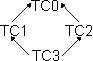
\includegraphics[width=0.62in]{figs/cloud_lattice.pdf}
            \caption{ A lattice governing the timing compartments of the cloud 
                computing environment. TC3 preceeds TC1 and TC2. TC1 and TC2 
                are incomparable with each other, but preceed TC0
            }
            \label{fig:cloud_lattice}
        \end{center}
    \end{figure}

    The lattice in Figure \ref{fig:cloud_lattice} defines the policy. TC3 
    preceeds both TC1 and TC2 implying timing channel leakage from VM3 or VM4 
    to any other VM is not controlled. However, VM1 and VM2 cannot leak 
    information to VM3 or VM4. Additionally, VM1 and VM2 cannot leak 
    information to each other since TC1 and TC2 are incomparable. All other TCs 
    preceed TC0, so leakage from any VM to the hypervisor is not controlled, 
    but the hypervisor cannot leak any information to the VMs.This meets the 
    security requirements of VM1 and VM2 since both are totally isolated from 
    the other VMs through timing channels. Since VM3 and VM4 share a timing 
    compartment, they can share resources normally and incur minimal 
    performance overheads.
